
%\chapter{TEORIA DE LA UTILIDAD}
%\chapter{MODELOS BAJO INCERTIDUMBRE}
%\chapter{TEORÍA DEL RIESGO Y ÁRBOLES DE DECISIÓN}
%\chapter{ANÁLISIS BAYESIANO}
%\section{}
%\subsection{}
%\chapter{TEORÍA DE JUEGOS}
%\chapter{REDES DE AUTÓMATAS ESTOCÁSTICOS}
%\chapter{DECISIONES MULTIOBJETIVO EN COMUNIDADES DE AGENTES ARTIFICIALES: COOPERACIÓN Y NEGOCIACIÓN}

\chapter{DECISIONES EN COMUNIDADES DE AGENTES ARTIFICIALES}

\begin{flushright}
\textit{"Vamos a intentar enseñar la generosidad y el altruismo, porque todos nacemos egoístas."}\\
\textbf{Richard Dawkins}
\end{flushright}

En este capítulo se exponen los principios de la teoría de juegos que permiten construir comunidades de agentes altruistas.  Los miembros de estas comunidades abandonan en alguna medida sus estructuras de preferencias y sus intereses individuales para decidir siempre en persecución  de los objetivos del grupo al cual pertenecen.

\section{INTRODUCCIÓN}
En términos generales, la autonomía de un agente artificial, esto es su capacidad de asumir decisiones racionales, puede  implementarse siguiendo uno de tres posibles enfoques. El primero de ellos es construir un \textbf{agente egoísta}, es decir aquel cuyas acciones deben orientarse a satisfacer su estructura de preferencias descrita mediante un modelo de utilidad individual.  El segundo, por el contrario, consiste en implementar un \textbf{agente altruista} que, como tal, abandona por completo sus intereses propios e individuales para tomar decisiones pensando exclusivamente en la comunidad a la cual pertenece. Un tercer (y más interesante) enfoque de diseño consiste en construir agentes que, sin ser completamente egoístas tampoco son, en absoluto, altruistas.  Este capítulo está dedicado a presentar las bases de la teoría de juegos sobre la cual pueden construirse comunidades de agentes altruistas.\\

En el diccionario de la Real Academia Española, se define al altruismo como aquella palabra que proviene del francés \textit{altruisme} y que significa “Diligencia en procurar el bien ajeno aún a costa del propio”.  Es precisamente esta acepción el punto de partida para diseñar comunidades de agentes altruistas.  Por esta razón, basados en la Teoría de Juegos, en este documento se presentan los principales resultados matemáticos que hacen posible la implementación de este tipo de grupos de agentes que se coordinan o que cooperan en persecución de uno o varios objetivos grupales abandonando sus propios intereses.  Aunque los postulados matemáticos se proponen para situaciones en las cuales actúan solamente dos agentes, vale advertir que dichos fundamentos se pueden (en la mayoría de los casos) extender fácilmente a grupos constituidos por tres o más agentes.  El resultado teórico más importante que se propone en este documento es el Teorema Fundamental de la teoría de juegos por ello todos los principios que se incluyen o bien lo fundamentan o bien lo complementan.  Se ha evitado dejar por fuera cualquier detalle teórico necesario pero, al mismo tiempo, se ha tenido especial cuidado en incluir sólo aquellos complementos realmente indispensables.\\

Para cumplir con los objetivos de este capítulo, primero se hace, en la sección \ref{Sec:Planteamiento},  el planteamiento del problema, luego se presenta en la sección \ref{Sec:Clas_JE} una clasificación de los juegos de estrategia.  Las principales secciones son la \ref{Sec:Juegos_SC2A} y la \ref{Sec:Juegos_SNC2A}, en las cuales se discuten con detalle el Teorema fundamentales de la teoría de juegos de suma constante y el Teorema fundamental de la teoría de juegos de suma no constante respectivamente.  Finalmente, a manera de ilustración, en la sección \ref{Sec:CE_DCA} se formulan y solucionan dos problemas que incluyen los usos de varias de las herramientas matemáticas presentadas.\\

\section{PLANTEAMIENTO DEL PROBLEMA}\label{Sec:Planteamiento}
La principal característica de los problemas de decisión que se enmarcan dentro de la teoría de juegos reside en el número  de agentes que son más de uno y que, usualmente, tienen intereses contrapuestos, razón por la cual se dice que el problema se encuentra en un ambiente de conflicto. Por lo tanto, en términos generales, en un juego de estrategias desempeñan un papel protagónico las acciones seguidas por el resto de los agentes.\\

Para iniciar con la discusión teórica, es necesario establecer los cuatro  \textbf{elementos de un juego de estrategia}:\\

\begin{enumerate}

\item \textit{Agentes}: El modelo supone la interacción de varios agentes decisores, a conjunto al  usualmente se denomina la comunidad de agentes.

\item \textit{Conjunto de alternativas}: Cada agente tendrá un conjunto de alternativas que podrá ser continuo o discreto.  Sin embargo, en este capítulo sólo presentarán problemas con conjunto de alternativas discretas. Al conjunto de alternativas del k-ésimo agente se denota como $A_k={\lbrace A^k_i \rbrace}_{i \in I} $ y $A^k_i$ será cada una de las alternativas de dicho agente. $A^k_i$ se les conoce también como estrategias (puras) del agente.

\item \textit{Estado de la naturaleza}: La variable de estado representa aquel factor o factores que influyen en el problema de decisión y que no están bajo el control del agente, es decir, es la variable que refleja el entorno del problema de decisión, a veces también conocida como contexto o entorno. Siendo más interesantes los entornos de naturaleza estocástica, en este documento se trabajará suponiendo un ambiente de certeza.

\item \textit{Criterio de evaluación}: Es una función que permite valorar el conjunto de alternativas o estrategias. La característica  esencial de los juegos de estrategia  reside precisamente en el hecho de  que el resultado que se deriva de la utilización de una determinada forma de actuar del agente, sino que también es consecuencia de las estrategias seguidas por el resto de los agentes. De esta manera, aplicar el criterio de  evaluación  dará lugar a lo que se conoce como función de pagos del agente. Cada agente tendrá entonces su propia función de pagos. Si, por ejemplo, el conjunto de estrategias de cada agente es finito y el número de agentes es dos, la función de pagos se puede representar en las llamadas matrices de pagos para cada uno de los agentes, de la siguiente manera:
\end{enumerate}


\setlength{\unitlength}{1cm}
\thicklines

\begin{figure}[h] % Flotante "comun",en que irán ambos
\begin{center}

\begin{picture}(6,6)
\put(0,5){\line(1,0){6}}
\put(1,0){\line(0,1){6}}
\put(0.25,4.5){$A_1$}
\put(0.25,3.5){$\vdots$}
\put(0.25,2.5){$A_i$}
\put(0.25,1.5){$\vdots$}
\put(0.25,0.5){$A_n$}

\put(1.25,5.5){$B_1$}
\put(1.25,4.5){$r_{11}^A$}
\put(1.25,3.5){$\vdots$}
\put(1.25,2.5){$r_{i1}^A$}
\put(1.25,1.5){$\vdots$}
\put(1.25,0.5){$r_{n1}^A$}

\put(2.25,5.5){$\cdots$}
\put(2.25,4.5){$\cdots$}
\put(2.25,3.5){$\ddots$}
\put(2.25,2.5){$\cdots$}
\put(2.25,1.5){$\ddots$}
\put(2.25,0.5){$\cdots$}

\put(3.25,5.5){$B_j$}
\put(3.25,4.5){$r_{1j}^A$}
\put(3.25,3.5){$\vdots$}
\put(3.25,2.5){$r_{ij}^A$}
\put(3.25,1.5){$\vdots$}
\put(3.25,0.5){$r_{nj}^A$}

\put(4.25,5.5){$\cdots$}
\put(4.25,4.5){$\cdots$}
\put(4.25,3.5){$\ddots$}
\put(4.25,2.5){$\cdots$}
\put(4.25,1.5){$\ddots$}
\put(4.25,0.5){$\cdots$}

\put(5.25,5.5){$B_m$}
\put(5.25,4.5){$r_{1m}^A$}
\put(5.25,3.5){$\vdots$}
\put(5.25,2.5){$r_{im}^A$}
\put(5.25,1.5){$\vdots$}
\put(5.25,0.5){$r_{nm}^A$}

\end{picture}

\end{center}

\begin{center}

\begin{picture}(6,6)
\put(0,5){\line(1,0){6}}
\put(1,0){\line(0,1){6}}
\put(0.25,4.5){$A_1$}
\put(0.25,3.5){$\vdots$}
\put(0.25,2.5){$A_i$}
\put(0.25,1.5){$\vdots$}
\put(0.25,0.5){$A_n$}

\put(1.25,5.5){$B_1$}
\put(1.25,4.5){$r_{11}^B$}
\put(1.25,3.5){$\vdots$}
\put(1.25,2.5){$r_{i1}^B$}
\put(1.25,1.5){$\vdots$}
\put(1.25,0.5){$r_{n1}^B$}

\put(2.25,5.5){$\cdots$}
\put(2.25,4.5){$\cdots$}
\put(2.25,3.5){$\ddots$}
\put(2.25,2.5){$\cdots$}
\put(2.25,1.5){$\ddots$}
\put(2.25,0.5){$\cdots$}

\put(3.25,5.5){$B_j$}
\put(3.25,4.5){$r_{1j}^B$}
\put(3.25,3.5){$\vdots$}
\put(3.25,2.5){$r_{ij}^B$}
\put(3.25,1.5){$\vdots$}
\put(3.25,0.5){$r_{nj}^B$}

\put(4.25,5.5){$\cdots$}
\put(4.25,4.5){$\cdots$}
\put(4.25,3.5){$\ddots$}
\put(4.25,2.5){$\cdots$}
\put(4.25,1.5){$\ddots$}
\put(4.25,0.5){$\cdots$}

\put(5.25,5.5){$B_m$}
\put(5.25,4.5){$r_{1m}^B$}
\put(5.25,3.5){$\vdots$}
\put(5.25,2.5){$r_{im}^B$}
\put(5.25,1.5){$\vdots$}
\put(5.25,0.5){$r_{nm}^B$}

\end{picture}
\end{center}
\end{figure} % Fin del entorno comun. No lleva caption

En esta representación matricial $r_{ij}^A$ es el pago que recibe $A$ cuando sigue la estrategia $A_i$, y el agente $B$ sigue la estrategia $B_j$ mientras que $r_{ij}^B$ es el pago que recibe el agente $B$ cuando el sigue la estrategia $B_j$ y el agente $A$ sigue la estrategia $A_i$. En lo que sigue se tratará con problemas en los cuales intervienen como máximo dos agentes; Sin embargo, vale decir que la extensión a mas de tres agentes decisores es directa y no implica mayores cambios en el planteamiento teórico expuesto.
\\

\section{CLASIFICACIÓN DE LOS JUEGOS DE ESTRATEGIA}\label{Sec:Clas_JE}
Existen muchas clasificaciones relacionadas con los juegos de estrategia. Prácticamente cada autor tiene las suyas. Parece haber, sin embargo, coincidencias en varias de ellas. Aquí se comentan las clasificaciones más reiteradas y usadas por la comunidad académica. Desde cierto punto de vista, estos criterios no son incompatibles entre sí, al contrario se complementan en la mayoría de los casos.
\\
\begin{enumerate}
\item \textbf{Criterio según el numero de agentes:} los juegos de estrategia pueden ser entre \textit{dos agentes} o bien \textit{juegos n-personales} o de \textit{n} agentes.
\item \textbf{Criterio según el numero de alternativas de cada agente:} Desde esta perspectiva hay \textit{Juegos discretos} los cuales son aquellos juegos en los que cada agente tiene un conjunto \textit{finito} de alternativas. En contraste, están los \textit{juegos con infinito número de alternativas}. En este último caso existe, de un lado, la subdivisión de juegos con infinito pero numerable conjunto de alternativas y de otro lado, los juegos continuos que son aquellos en los que cada agente cuenta con un conjunto infinito (no numerable) de alternativas.
\item \textbf{Criterio según la información disponible:} \textit{Juegos con información completa:} Cada agente conoce perfectamente la función de pagos de todos los agentes. \textit{Juegos con información incompleta:} Algún agente no conoce completamente la función de pagos de otro u otros agentes. Así mismo, la información puede ser: \textit{Perfecta:} si es de carácter cierto o bien \textit{Imperfecta:} si es de carácter aleatorio.
\item \textbf{Criterio según la forma en la que se toma la desición:} De esta manera se tienen \textit{Juegos estáticos:} Las decisiones son tomadas de forma simultánea por todos los agentes. \textit{Juegos dinámicos:} las decisiones por los agentes de manera secuencial.
\item \textbf{Criterio según la existencia de comunicación previa entre los agentes:} Los juegos pueden ser \textit{cooperativos} cuando existe comunicación entre los agentes antes de tomar la decisión o bien \textit{juegos no cooperativos} cuando no existe comunicación entre los agentes antes de tomar la decisión.
\item \textbf{Criterio según la función de pagos:} Es, desde el punto de vista de este capítulo la clasificación mas importante. Desde este punto de vista, los juegos pueden ser \textit{de suma constante} cuando la suma de los pagos de los distintos agentes es constante, sea cual sea la combinación de estrategias seguida por cada agente o bien \textit{de suma no constante} en aquellas situaciones en las cuales la suma de los pagos de los distintos agentes no es siempre la misma, depende de la combinación de alternativas de cada agente.
\end{enumerate}
Existen otros criterios que llevan otras clasificaciones; sin embargo, las anteriores seis son suficientes para los propósitos de este documento.

\section{JUEGOS DE SUMA CONSTANTE ENTRE DOS AGENTES}\label{Sec:Juegos_SC2A}

Los juegos de suma constante se realizan entre dos agentes, presentan varias características importantes entre las cuales se destacan las siguientes: Pueden ser discretos o continuos. Aunque el tratamiento tiene muchas similitudes, en este documento se abordarán únicamente aquellos juegos de naturaleza \textit{discreta}. Así mismo, son juegos de \textit{información completa (también conocidos como juegos de información perfecta)}, debido a que los agentes conocen con certeza la función de pagos de todos los agentes que hacen parte de su comunidad. Claramente son situaciones que pocas veces se presentan en la realidad, pero con algo de trabajo adicional, es posible extender la teoría que se presentará a situaciones mas realistas y, por eso mismo, complejas.
\\
También son juegos \textit{estáticos}, es decir, las decisiones se toman simultáneamente por los dos agentes. Pero también son juegos \textit{no cooperativos}, esto es, no existe comunicación previa entre los agentes. Adicionalmente son juegos de \textit{suma constante}. La suma de los pagos de los distintos agentes es una determinada constante $C$, sea cual sea la estrategia seguida por cada agente. Esto puede interpretarse o pensarse como que los agentes compiten o actúan por repartirse esa cantidad $C$. En este caso las matrices de los agentes serán de la forma:
\\
 
 \begin{figure}[h] % Flotante "comun", sin caption, en que irán ambos
\begin{minipage}{0.45\textwidth} 
\begin{center}

\begin{picture}(6,6)
\put(0,5){\line(1,0){6}}
\put(1,0){\line(0,1){6}}
\put(0.25,4.5){$A_1$}
\put(0.25,3.5){$\vdots$}
\put(0.25,2.5){$A_i$}
\put(0.25,1.5){$\vdots$}
\put(0.25,0.5){$A_n$}

\put(1.25,5.5){$B_1$}
\put(1.25,4.5){$r_{11}^A$}
\put(1.25,3.5){$\vdots$}
\put(1.25,2.5){$r_{i1}^A$}
\put(1.25,1.5){$\vdots$}
\put(1.25,0.5){$r_{n1}^A$}

\put(2.25,5.5){$\cdots$}
\put(2.25,4.5){$\cdots$}
\put(2.25,3.5){$\ddots$}
\put(2.25,2.5){$\cdots$}
\put(2.25,1.5){$\ddots$}
\put(2.25,0.5){$\cdots$}

\put(3.25,5.5){$B_j$}
\put(3.25,4.5){$r_{1j}^A$}
\put(3.25,3.5){$\vdots$}
\put(3.25,2.5){$r_{ij}^A$}
\put(3.25,1.5){$\vdots$}
\put(3.25,0.5){$r_{nj}^A$}

\put(4.25,5.5){$\cdots$}
\put(4.25,4.5){$\cdots$}
\put(4.25,3.5){$\ddots$}
\put(4.25,2.5){$\cdots$}
\put(4.25,1.5){$\ddots$}
\put(4.25,0.5){$\cdots$}

\put(5.25,5.5){$B_m$}
\put(5.25,4.5){$r_{1m}^A$}
\put(5.25,3.5){$\vdots$}
\put(5.25,2.5){$r_{im}^A$}
\put(5.25,1.5){$\vdots$}
\put(5.25,0.5){$r_{nm}^A$}

\end{picture}

\end{center}
\end{minipage} % Fin de la minipagina de la tabla
\hfill % Espacio flexible para separar tabla y figura
\begin{minipage}{0.45\textwidth} 
\begin{center}

\begin{picture}(6,6)
\put(0,5){\line(1,0){6}}
\put(1,0){\line(0,1){6}}
\put(0.25,4.5){$A_1$}
\put(0.25,3.5){$\vdots$}
\put(0.25,2.5){$A_i$}
\put(0.25,1.5){$\vdots$}
\put(0.25,0.5){$A_n$}

\put(1.25,5.5){$B_1$}
\put(1.25,4.5){$r_{11}^B$}
\put(1.25,3.5){$\vdots$}
\put(1.25,2.5){$r_{i1}^B$}
\put(1.25,1.5){$\vdots$}
\put(1.25,0.5){$r_{n1}^B$}

\put(2.25,5.5){$\cdots$}
\put(2.25,4.5){$\cdots$}
\put(2.25,3.5){$\ddots$}
\put(2.25,2.5){$\cdots$}
\put(2.25,1.5){$\ddots$}
\put(2.25,0.5){$\cdots$}

\put(3.25,5.5){$B_j$}
\put(3.25,4.5){$r_{1j}^B$}
\put(3.25,3.5){$\vdots$}
\put(3.25,2.5){$r_{ij}^B$}
\put(3.25,1.5){$\vdots$}
\put(3.25,0.5){$r_{nj}^B$}

\put(4.25,5.5){$\cdots$}
\put(4.25,4.5){$\cdots$}
\put(4.25,3.5){$\ddots$}
\put(4.25,2.5){$\cdots$}
\put(4.25,1.5){$\ddots$}
\put(4.25,0.5){$\cdots$}

\put(5.25,5.5){$B_m$}
\put(5.25,4.5){$r_{1m}^B$}
\put(5.25,3.5){$\vdots$}
\put(5.25,2.5){$r_{im}^B$}
\put(5.25,1.5){$\vdots$}
\put(5.25,0.5){$r_{nm}^B$}

\end{picture}
\end{center}
\end{minipage} % Fin de la minipagina que lleva la foto
\end{figure} % Fin del entorno comun. No lleva caption

\begin{center}
Con $r_{ij}^A + r_{ij}^B = C \quad \forall i,j$\\
\end{center}
En consecuencia, $ r_{ij}^B = C - r_{ij}^A $ para todo $i,j$. De esta manera, dado el pago para el agente $A$, el pago para el agente $B$ es también conocido. Estos supuestos hacen que en este tipo de juegos solamente se requiera una matriz de pagos para modelarlos.
\\
Claramente, un caso particular de los juegos de suma constante son los juegos de suma nula, en los que la cosntante $C=0$. En este caso $ r_{ij}^B = - r_{ij}^A \quad \forall i,j$, es decir, lo que gana o cobra el otro agente es exactamente lo que pierde o paga el otro agente. En los juegos de suma constante, copmo se comentó antes, se requiere una única matriz de pagos, la del agente $A$, que se denota por:

\begin{figure}[h]
\begin{center}
\begin{picture}(6,6)
\put(0,5){\line(1,0){6}}
\put(1,0){\line(0,1){6}}
\put(0.25,4.5){$A_1$}
\put(0.25,3.5){$\vdots$}
\put(0.25,2.5){$A_i$}
\put(0.25,1.5){$\vdots$}
\put(0.25,0.5){$A_n$}

\put(1.25,5.5){$B_1$}
\put(1.25,4.5){$r_{11}$}
\put(1.25,3.5){$\vdots$}
\put(1.25,2.5){$r_{i1}$}
\put(1.25,1.5){$\vdots$}
\put(1.25,0.5){$r_{n1}$}

\put(2.25,5.5){$\cdots$}
\put(2.25,4.5){$\cdots$}
\put(2.25,3.5){$\ddots$}
\put(2.25,2.5){$\cdots$}
\put(2.25,1.5){$\ddots$}
\put(2.25,0.5){$\cdots$}

\put(3.25,5.5){$B_j$}
\put(3.25,4.5){$r_{1j}$}
\put(3.25,3.5){$\vdots$}
\put(3.25,2.5){$r_{ij}$}
\put(3.25,1.5){$\vdots$}
\put(3.25,0.5){$r_{nj}$}

\put(4.25,5.5){$\cdots$}
\put(4.25,4.5){$\cdots$}
\put(4.25,3.5){$\ddots$}
\put(4.25,2.5){$\cdots$}
\put(4.25,1.5){$\ddots$}
\put(4.25,0.5){$\cdots$}

\put(5.25,5.5){$B_m$}
\put(5.25,4.5){$r_{1m}$}
\put(5.25,3.5){$\vdots$}
\put(5.25,2.5){$r_{im}$}
\put(5.25,1.5){$\vdots$}
\put(5.25,0.5){$r_{nm}$}

\end{picture}
\end{center}
\end{figure} 

De esta manera, $r_{ij}$ es la cantidad que gana o cobra el agente $A$. ($r_{ij}$ resultado favorable para el agente $A$) y $C - r_{ij}$, será la cantidad que gana o cobra el agente $B$, luego $C-r_{ij}$ será la cantidad que <<gana o pierde>> $B$, ($r_{ij}$ resultado desfavorable para el agente $B$) cuando $A$ utiliza la estrategia $A_i$ y el agente $B$ utiliza la estrategia $B_j$.
\\
La filosofía o, mas formalmente, la racionalidad que emplean los agentes para elegir su estrategia óptima es una \textit{racionalidad prudente}, (en esto hay una gran distancia con los métodos para construir agentes egoístas en los cuales se habla de maximizar la utilidad esperada), dado que estos juegos se basan en el principio de que << el adversario es almenos tan inteligente como yo>>. En consecuencia, el objetivo de los agentes ya no es conseguir el resultado óptimo (de su utilidad) porque el contrincante no se lo va a permitir (puesto que el contexto es hostil), sino que cada uno de los agentes tratrá de evitar los peores resultados que se le puedan presentar. Eso llevaráal agente $A$ a utilizar su estrategia maximin y al agente $B$ utilizar su estrategia minimax:
\begin{center}
Agente A: $A^* \: \rightarrow \: \underset{i}{\max}\left( \underset{j}{\min} \: r_{ij} \right) $
\end{center}

la cantidad puede ser interpretada como la cantidad mínima que el jugardor $A$ está dispuesto a cobrar o ganar en el juego, es decir, con la cantidad mínima con la que el agente $A$ se conforma.
\\
\begin{center}
Agente A: $B^* \: \rightarrow \: \underset{i}{\min}\left( \underset{j}{\max} \: r_{ij} \right) $
\end{center}

La cantidad $C \: - \: \underset{i}{\min}\left( \underset{j}{\max} \: r_{ij} \right) $ se puede interpretar como la cantidad mínima que el agente B está dispuesto a recibir en el juego, es decir, la cantidad mínima con la que se conforma. Si el juego es de suma nula, la cantidad $\underset{i}{\min}\left( \underset{j}{\max} \: r_{ij} \right)$ se puede concebir, en consecuencia, como la cantidad máxima que el agente $B$ está dispuesto a perder o pagar.
\subsection{Estrategias dominadas}

Sea $J$ un juego de suma constante entre dos agentes  $A$ y $B$, de cuyas estrategias son $A_1,\cdots , A_n$ y $ B_1, \cdots , B_m$ para cada uno de los agentes respectivamente y matriz de pagos $\left( r_{ij}\right)_{i=1, \cdots ,n}^{j=1, \cdots, m} $

\theoremstyle{definicion}
\newtheorem{definicion}{Definición}
\begin{definicion}\label{Def:Comb_lin_conv}
\textbf{Combinación lineal convexa}
Se dice que $C^A$ es una combinación lineal convexa de estrategias puras de A si puede expresarse de la forma $C^A = \underset{i}{\sum}\alpha_i A_i$ con $\alpha_i \in \left[ 0,1 \right]$ y $\underset{i}{\sum} \alpha_i = 1$.\\
Los resultados (favorables) que el agente $A$ obtiene con esta estrategia  serán $\left( C_1, \cdots, c_j, \cdots, C_m\right)$ con $c_j = \underset{i}{\sum}\alpha_i r_{ij}$ De forma similar, $C_B$ es una combinación lineal convexa de estrategias puras de $B$ si puede expresarse de la forma $C^B = \underset{j}{\sum}\lambda_j B_j$ para $\lambda_j \in  \left[ 0,1 \right]$ y $\underset{j}{\sum}\lambda_j = 1$ .  También en este caso Los resultados (desfavorables) que $B$ obtiene con esta estrategia serán $\left( C_1, \cdots, c_i, \cdots, C_m\right)$ con $c_i = \underset{j}{\sum}\alpha_i r_{ij}$
\end{definicion}

\begin{definicion}\label{Def:Dom_estra}
\textbf{Dominación de estrategias.}
Se dice que la estrategia pura $A_s$, domina a la estrategia pura $A_k$ (o lo que es lo mismo, $A_k$ está dominada por la estrategia pura $A_s$)  para el agente $A$ si los resultados (o pagos) que $A$ consigue con  son siempre mayores o iguales a los que consigue con $A_k$.  Formalmente, ello quiere decir que se verifica:
\begin{center}
    $r_{sj} \geq r_{kj} \forall j \quad  $ y $\exists j_0 \: r_{sj_0} > r_{kj_0}$
\end{center}
Análogamente, puede decirse la estrategia pura $B_s$, domina a la estrategia pura $B_k$ (o en otras palabras, $B_k$ está dominada por la estrategia pura $B_s$)  para el agente $B$ si los resultados (pagos) que $B$ consigue con  son siempre mayores o iguales a los que consigue con $B_k$.  Esto es, matemáticamente, que: 
\begin{center}
    $ r_{is} \geq r_{ik} \forall i \quad  $ y $\exists i_0 \: r_{is_0} > r_{ik_0}$
\end{center}
La combinación convexa de las estrategias de $A$, $C^A = \underset{i\in k}{\sum}\alpha_i A_i$  domina a la estrategia pura $A_k$ (esto es, $A_k$ está dominada por la estrategia pura $C^A$)  para el agente $A$ si los resultados (o, si se quiere, cobros) que $A$ consigue con $C^A$ son siempre mayores o iguales a los que consigue con $A_k$.  Equivalentemente:
\begin{center}
    $ c_j \geq r_{kj} \forall j \quad  $ y $\exists j_0 \: c_{j_0} > r_{kj_0}$
\end{center}
Por su parte, se dice que la combinación convexa de las estrategias de $B$, $C^B = \underset{j\in k}{\sum}\lambda_j B_j$ domina a la estrategia pura $B_k$ (o en otras palabras, $B_k$ está dominada por la estrategia pura $C^B$)  para el agente $B$ si los resultados (cobros) que $B$ consigue con $C^B$ son mayores o iguales a los que consigue con $B_k$, o, lo que es lo mismo:
\begin{center}
    $ c_i \geq r_{ik} \forall i \quad  $ y $\exists i_0 \: c_{i_0} > r_{ik_0}$
\end{center}
En aquellas situaciones en las cuales las desigualdades anteriores son estrictas (excluyen la igualdad), la dominación se dice estricta.  Estas definiciones permiten especular razonablemente por la veracidad del postulado que sigue.
\end{definicion}
\newtheorem{proposicion}{Proposición}
\begin{proposicion}
Un agente racional nunca utilizará una estrategia estrictamente dominada en su estrategia óptima.
\end{proposicion}

\subsection{Solución de un juego de suma constante entre dos agentes}
Conviene formular, antes de postular  la solución pura de un juego, la proposición que sigue cuya validez parece no admitir dudas:
\begin{proposicion}
Sea $J$ un juego de suma constante entre dos agentes $A$ y $B$ de estrategias $A_1, \cdots, A_n$ y $B_1, \cdots, B_m$  respectivamente y matriz de pagos $\left(r_{ij}\right)_{i=1, \cdots ,n}^{j=1, \cdots, m} $ Entonces $\underset{i}{\max}\left( \underset{j}{\min} \: r_{ij} \right) \leq \underset{i}{\min}\left( \underset{j}{\max} \: r_{ij} \right)$ .  Con frecuencia se dice que un juego de suma constante entre dos agentes tiene \textbf{solución pura} o \textbf{equilibrio puro} cuando  $\underset{i}{\max}\left( \underset{j}{\min} \: r_{ij} \right) = \underset{i}{\min}\left( \underset{j}{\max} \: r_{ij} \right)$
\end{proposicion}

La solución del juego, en este caso, es una terna $\left( A^*,B^*,v \right)$ en la cual $v = \underset{i}{\max}\left( \underset{j}{\min} \: r_{ij} \right) = \underset{i}{\min}\left( \underset{j}{\max} \: r_{ij} \right)$ se conoce como el \textbf{valor del juego}, $A^*$ es la estrategia pura óptima de $A$ y $B^*$ es la estrategia pura óptima de $B$, de forma que la función de pagos para $A_i = A^*$ y $B_j=B^*$ es v.
\\
En palabras relativamente sencillas, la existencia de solución pura en un juego se puede interpretar de la siguiente manera: el agente $A$ siempre utilizará la estrategia $A^*$, el agente $B$ siempre utilizará $B^*$ y el valor del juego siempre será $v$, que se interpreta como la cantidad  que el agente $A$ paga y, por tanto, $C-v$ será la cantidad que gana el agente $B$. Si el juego es de suma nula $(C=0)$, $v$ se interpreta como la cantidad que gana o pierde el agente $B$.

\newtheorem{definicion}{Definición}
\begin{definicion}\label{Def:Pto_silla_mp}
\textbf{Punto de silla de una matriz de pagos.}
Sea $J$ un juego bipersonal de suma constante, con agentes $A$ y  $B$ de estrategias $A_1, \cdots, A_n$ y $B_1, \cdots, B_m$ respectivamente y la matriz de pagos $\left( r_{ij}\right)_{i=1, \cdots ,n}^{j=1, \cdots, m}$.  La función de pagos tiene un \textbf{punto de silla} si existe un pago que es simultáneamente mínimo de una fila y máximo de una columna, es decir:

\begin{center}
    $\exists i_0,j_0 \: | \: \begin{cases}
    r_{i_0j} \geq r_{i_0,j_0}, & \forall j = 1,2,\cdots,m.\\
    r_{ij_0} \leq r_{i_0,j_0}, & \forall i = 1,2,\cdots,n.
  \end{cases}$
\end{center}
\end{definicion}


\begin{proposicion}
La condición necesaria y suficiente para que un juego de suma constante entre dos agentes tenga solución pura es que su función de pagos tenga un punto de silla.
\end{proposicion}

\subsection{Solución mixta de un juego bipersonal de suma constante}
Un juego de suma constante entre dos agentes no siempre tiene solución pura. Esta falta de equilibrio lleva a los agentes a tratar de engañar a su contrario no utilizando siempre su misma estrategia. Ello implica que, si el juego se repitiese sucesivas veces, cada uno de los agentes emplearía sus estrategias puras con distinta probabilidad, es decir, aleatorizaría  sus estrategias. 
\\
Sea $J$  un juego de suma constante entre dos agentes  $A$ y $B$ de estrategias $A_1, \cdots, A_n$ y $B_1, \cdots, B_m$ para cada uno de los agentes respectivamente y matriz de pagos $\left( r_{ij}\right)_{i=1, \cdots ,n}^{j=1, \cdots, m}$

\begin{definicion}\label{Def:Estr_mix}
\textbf{Estrategia mixta de los agentes}
\begin{enumerate}
    \item Una  \textbf{estrategia mixta para el agente A} es una distribución de probabilidad asociada a su conjunto de estrategias puras, en otras palabras, $P = (p_1,\ldots,p_i, \ldots,p_n)$ con $p_i \in [0,1]$ y $\underset{i}{\sum}p_i = 1$ donde los $p_i$ representa la probabilidad de que el agente A utilice la estrategia $A_i$
    \item Una  estrategia mixta para el agente $B$ es una distribución de probabilidad asociada a su conjunto de estrategias puras, es decir, $Q = (q_1,\ldots,q_j,\ldots,q_m)$ con $q_j \in [0,1]$ y $\underset{j}{\sum}q_j = 1$ donde los  representa la probabilidad de que el agente B utilice la estrategia $B_j$
\end{enumerate}
\end{definicion}

\begin{definicion}\label{Def:Fun_pag_esp}
\textbf{Función de pago esperado.}
\begin{enumerate}
    \item Se define la esperanza del agente $A$ condicionado a que el agente $B$ utilice su estrategia $B_j$ y notamos, $E(A|B_j)$, como:
    \begin{center}
        $E(A|B_j) = p_1r_{1j}+\ldots+p_ir_{ij}+\ldots+p_nr_{nj} = \underset{i}{\sum}p_ir_{ij}$
    \end{center}
     $E(A|B_j)$representa la cantidad que el agente $A$ espera ganar si utiliza su estrategia mixta $P$ y el agente $B$ utiliza su estrategia $B_j$.
     
    \item De forma similar, se define  la esperanza del agente $B$ condicionado a que el agente $A$ utilice su estrategia $A_i$ y notamos, $E(B|A_i)$ como:
    \begin{center}
        $E(B|A_i) = q_1r_{i1}+\ldots+q_jr_{ij}+\ldots+q_mr_{im} = \underset{j}{\sum}q_jr_{ij}$
    \end{center}
    $C-E(B|A_i)$ representa la cantidad que el agente $A$ espera ganar si utiliza su estrategia mixta $Q$  y el agente $A$ utiliza su estrategia $A_i$. Además, si el juego es de suma nula $E(B|A_i)$ representa la cantidad que el agente $B$ espera pagar o perder si el agente $A$ utiliza su estrategia $A_i$.
\end{enumerate}
\end{definicion}

\begin{definicion}\label{Def:Func_esp_j}
\textbf{Función de esperanza del juego.}
La función esperanza de juego, denotada como $E(P,Q)$ se define mediante la expresión:
\begin{center}
    $E(P,Q) = \underset{j}{\sum}E(A|B_j)q_i = \underset{i}{\sum}E(B|A_i)p_i = \underset{i}{\sum}\underset{j}{\sum}r_{ij}p_i q_j$
\end{center}
$E(P,Q)$ representa la cantidad que el agente A espera ganar si utiliza su estrategia mixta P y B utiliza su estrategia mixta Q, mientras $C-E(P,Q)$ representa la cantidad que el agente B espera ganar si utiliza su estrategia mixta Q y A utiliza su estrategia mixta P. Cuando el juego es de suma nula $(C=0)$ la cantidad  representa la cantidad que el agente B espera ganar o perder sea cual sea la estrategia que emplee el agente A.
\\
De esta manera, los agentes utilizarán aquella estrategia que:
\begin{center}
   Agente A: $A^* \rightarrow \underset{P}{\max}\left[ \underset{Q}{\min} \: E(P,Q) \right] $ \\
   Agente B: $B^* \rightarrow \underset{Q}{\min}\left[ \underset{P}{\max} \: E(P,Q) \right]  $
\end{center}
\end{definicion}

\begin{definicion}
\textbf{Solución mixta.}
Se dice que un juego de suma constante entre dos agentes tiene solución mixta o equilibrio mixto si se cumple que:
\begin{center}
    $ \underset{P}{\max}\left[ \underset{Q}{\min} \: E(P,Q) \right] = \underset{Q}{\min}\left[ \underset{P}{\max} \: E(P,Q) \right] $
\end{center}
En este caso, la solución del juego es una terna $(P^*,Q^*,v)$ donde:
\begin{center}
    $ v = \underset{P}{\max}\left[ \underset{Q}{\min} \: E(P,Q) \right] = \underset{Q}{\min}\left[ \underset{P}{\max} \: E(P,Q) \right] $
\end{center}
El valor del juego, $P^* = (p_1^*,\ldots,p_i^*,\ldots,p_n^*)$ es la estrategia óptima de $A$ y $Q^* = (q_1^*,\ldots,q_j^*,\ldots,q_m^*)$ es la estrategia mixta óptima de $B$, tales que $v=E(P^*,Q^*)$.  La solución mixta se puede interpretar de la siguiente manera:
\\
En cada una de las repeticiones del juego, el agente $A$ utiliza una de sus estrategias puras, por lo tanto, si el juego se repite sucesivas veces, cada estrategia pura $A_i$ es utilizada por el agente $A$ con una probabilidad $p_i^*$; mientras el agente $B$ utiliza una de sus estrategias puras, por lo tanto, si el juego se repite sucesivas veces, cada estrategia pura $B_j$ es utilizada por el agente $B$ con una probabilidad $q_j^*$. El valor del juego $v=E(P^*,Q^*)$ Representa la cantidad que el agente $A$ espera ganar, de media, si se enfrenta sucesivas veces al agente B en el juego. La  cantidad $(C-v)$ representa a la cantidad que el agente $B$ espera ganar, de media, si se enfrenta sucesivas veces al agente $A$ en el juego. Si el juego es de suma nula $(C=0)$, $v = E(P^*,Q^*)$ representa la cantidad que el agente $B$ espera perder o pagar, de media, si se enfrenta sucesivas veces al agente $A$ en el juego.
\end{definicion}

\begin{proposicion}
La condición necesaria y suficiente para que un juego de suma constante entre dos agentes tenga solución mixta es que la función esperanza de juego tenga un punto de silla.
\end{proposicion}

\begin{theorem}
\textbf{Teorema fundamental de la teoría de juegos.}
En un juego de suma constante entre dos agentes, la función esperanza del juego siempre tiene, al menos, un punto de silla, es decir:
\begin{center}
    $\underset{P}{\max}\left[ \underset{Q}{\min} \: E(P,Q) \right] = \underset{Q}{\min}\left[ \underset{P}{\max} \: E(P,Q) \right] = E(P^*,Q^*)$
\end{center}
En consecuencia, todo juego de suma constante entre dos agentes tiene solución.
\end{theorem}

En todo  juego de suma constante $C$ entre dos agentes se puede demostrar que:
\begin{enumerate}
    \item $E(A|B_j) \geq v=E(P^*,Q^*)$
    \item $E(B|A_i) \leq v= E(P^*,Q^*)$
    \item $E(P,Q^*) \leq E(P^*,Q^*) \leq E(P^*,Q)$
    \item $\underset{i}{\max}\left[ \underset{j}{\min} \: r_{ij} \right]  \leq E(P^*,Q^*) \leq \underset{j}{\min}\left[ \underset{i}{\max} \: r_{ij} \right]$
\end{enumerate}


\subsection{Modelo de programación lineal para juegos de suma constante}

Hasta este momento se ha propuesto que todo juego de suma constante entre dos agentes tiene solución. Sin embargo, todavía no se ha propuesto algún método que permita el cálculo de tal solución. Los \textbf{métodos habituales de resolución de un juego} de este tipo son, fundamentalmente, dos:

\begin{enumerate}
    \item \textbf{El método gráfico.} Es un método muy  sencillo pero, a la vez, muy limitado puesto que tiene el inconveniente de que solo es aplicable cuando al menos uno de los dos agentes utiliza un máximo de dos estrategias puras, puesto que ello permite representar en el plano las funciones de pago esperado. El desarrollo de este método puede verse en los casos de estudio resueltos más adelante.
    \item \textbf{La solución del modelo de programación lineal asociado a todo juego.} Este método es más abstracto que el anterior, puesto que conlleva la solución de, al menos, un modelo de programación lineal. Pero es, en cambio, un método más general, puesto que es aplicable a cualquier juego de suma constante entre dos agentes. Este es el método que se expone  a continuación.
    \item \textbf{La solución del modelo de programación dinámica asociado a todo juego.} Este método es el más completo de los tres puesto que tiene mayor flexibilidad sin embargo, en la mayoría de situaciones no se hace necesario su uso debido a la linealidad supuesta en todos los planteamientos teóricos desarrollados hasta este momento.  Modelos de agentes más complejos pueden quitar los supuestos de linealidad caso en el cual la programación lineal no sería aplicable y quedaría como último recurso esta herramienta matemática para encontrar la solución.
\end{enumerate}

Existen otros métodos que pueden ser empleados (y seguramente con mayor eficiencia) sin embargo, ellos se salen del alcance de este capítulo.

\begin{proposicion}
Sea J un juego de suma constante entre los agentes A y B de estrategias $A_1,\ldots,A_n$ y $B_1,\ldots,B_m$ para cada uno de los agentes respectivamente y matriz de pagos $\left( r_{ij}\right)_{i=1, \cdots ,n}^{j=1, \cdots, m}$. Sea $J'$ un juego de suma constante entre los agentes A y B de estrategias $A_1,\ldots,A_n$ y $B_1,\ldots,B_m$ para cada uno de los agentes respectivamente y matriz de pagos con una constante real k cualquiera. Entonces las estrategias óptimas de cada uno de los agentes de cada uno es la misma en el juego J y en el juego  Además, si v es el valor del juego J entonces el valor del juego $J'$ es $v' = v+k$
\end{proposicion}

\begin{proposicion}
Sea J un juego de suma constante C, entre los agentes A y B de estrategias puras $A_1,\ldots,A_n$ y $B_1,\ldots,B_m$ para cada uno de los agentes respectivamente y matriz de pagos $\left( r_{ij}\right)_{i=1, \cdots ,n}^{j=1, \cdots, m}$ . Sean $P=(p_1,\ldots,p_i,\ldots,p_n)$ y $Q=(q_1,\ldots,q_j,\ldots,q_m)$ las estrategias mixtas de los agentes A  y B respectivamente. Sea $v>0$ el valor del juego. Entonces, los programas lineales asociados a los agentes A y B respectivamente se construyen de la forma:\\

\begin{minipage}{0.45\textwidth}
Agente A:\\
$\max \: v$
    \begin{align*}
    s.a \: E(A|B_j) \geq v \: \forall j =1,\ldots,m \\
    p_1+\ldots+p_i+\ldots+p_n = 1 \\
    p_i \geq 0 , \:v \geq 0\\
    \end{align*}
\end{minipage}
\begin{minipage}{0.45\textwidth}
Agente B:\\
$\min \: v$
    \begin{align*}
    s.a \: E(A|B_j) \geq v \: \forall j =1,\ldots,m \\
    p_1+\ldots+p_i+\ldots+p_n = 1 \\
    p_i \geq 0 , \:v \geq 0\\
    \end{align*}
\end{minipage}

Desarrollando estas expresiones, se obtienen los siguientes \textit{programas duales} para cada uno de los agentes:\\

\begin{minipage}{0.45\textwidth}
Agente A:\\
$\min \: x_1+\ldots+x_i+\ldots+x_n$\\
s.a 
    \begin{align*}
    r_{11}x_1+\ldots+r_{i1}x_i+\ldots+r_{n1}x_n  \geq 1\\
    r_{1j}x_1+\ldots+r_{ij}x_i+\ldots+r_{nj}x_n  \geq 1\\
    r_{1m}x_1+\ldots+r_{im}x_i+\ldots+r_{nm}x_n \geq 1\\
    \end{align*}
$x_i \geq 0$\\
\end{minipage}
\begin{minipage}{0.45\textwidth}
Agente B:\\
$\max \: y_1+\ldots+y_j+\ldots+y_m$\\
s.a 
    \begin{align*}
    r_{11}y_1+\ldots+r_{i1}y_j+\ldots+r_{1m}y_m  \geq 1\\
    r_{1j}y_1+\ldots+r_{ij}y_j+\ldots+r_{im}y_m  \geq 1\\
    r_{1m}y_1+\ldots+r_{im}y_j+\ldots+r_{nm}y_m \geq 1\\
    \end{align*}
$y_j \geq 0$ \\
\end{minipage}

Donde $x_i = \frac{p_i}{v} \geq 0, \: y_j = \frac{q_j}{v} \geq 0$ y $v=\frac{1}{x_1+\ldots+x_i+\ldots+x_n} = \frac{1}{y_1+\ldots+y_j+\ldots+y_m}$
\\
Si antes de empezar a plantear el programa lineal de cada agente no puede garantizarse el cumplimiento de la condición $v>0$, es necesario sumar  una constante suficientemente grande a la matriz de pagos (para que todos los pagos sean positivos), construiremos y resolveremos  los programas lineales para el problema transformado y, en virtud de la proposición anterior, determinaremos la solución del programa inicial.

\end{proposicion}

\section{JUEGOS DE SUMA NO CONSTANTE ENTRE DOS AGENTES}\label{Sec:Juegos_SNC2A}

Dentro de los juegos de suma no constante o variable entre dos agentes y donde la suma de los pagos de los distintos agentes depende de la estrategia seguida por cada uno de ellos, se presentarán los fundamentos teóricos bajo los siguientes supuestos:  (1) Son juegos \textit{discretos}, (2) Son juegos de \textit{información completa y perfecta}, es decir, los agentes conocen con certeza la función de pagos de todos los agentes, (3) Son juegos \textit{estáticos}, debido a que las decisiones se toman simultáneamente por los dos agentes, (4) Corresponden a juegos  \textit{no cooperativos}, es decir, no existe comunicación previa entre los agentes y, finalmente,  (5) son juegos de  \textit{suma variable}. En este caso las matrices de pagos para los agentes toma  la forma:

\begin{figure}[h] % Flotante "comun", sin caption, en que irán ambos
\begin{minipage}{0.45\textwidth} 
\begin{center}

\begin{picture}(6,6)
\put(0,5){\line(1,0){6}}
\put(1,0){\line(0,1){6}}
\put(0.25,4.5){$A_1$}
\put(0.25,3.5){$\vdots$}
\put(0.25,2.5){$A_i$}
\put(0.25,1.5){$\vdots$}
\put(0.25,0.5){$A_n$}

\put(1.25,5.5){$B_1$}
\put(1.25,4.5){$r_{11}^A$}
\put(1.25,3.5){$\vdots$}
\put(1.25,2.5){$r_{i1}^A$}
\put(1.25,1.5){$\vdots$}
\put(1.25,0.5){$r_{n1}^A$}

\put(2.25,5.5){$\cdots$}
\put(2.25,4.5){$\cdots$}
\put(2.25,3.5){$\ddots$}
\put(2.25,2.5){$\cdots$}
\put(2.25,1.5){$\ddots$}
\put(2.25,0.5){$\cdots$}

\put(3.25,5.5){$B_j$}
\put(3.25,4.5){$r_{1j}^A$}
\put(3.25,3.5){$\vdots$}
\put(3.25,2.5){$r_{ij}^A$}
\put(3.25,1.5){$\vdots$}
\put(3.25,0.5){$r_{nj}^A$}

\put(4.25,5.5){$\cdots$}
\put(4.25,4.5){$\cdots$}
\put(4.25,3.5){$\ddots$}
\put(4.25,2.5){$\cdots$}
\put(4.25,1.5){$\ddots$}
\put(4.25,0.5){$\cdots$}

\put(5.25,5.5){$B_m$}
\put(5.25,4.5){$r_{1m}^A$}
\put(5.25,3.5){$\vdots$}
\put(5.25,2.5){$r_{im}^A$}
\put(5.25,1.5){$\vdots$}
\put(5.25,0.5){$r_{nm}^A$}

\end{picture}

\end{center}
\end{minipage} % Fin de la minipagina de la tabla
\hfill % Espacio flexible para separar tabla y figura
\begin{minipage}{0.45\textwidth} 
\begin{center}

\begin{picture}(6,6)
\put(0,5){\line(1,0){6}}
\put(1,0){\line(0,1){6}}
\put(0.25,4.5){$A_1$}
\put(0.25,3.5){$\vdots$}
\put(0.25,2.5){$A_i$}
\put(0.25,1.5){$\vdots$}
\put(0.25,0.5){$A_n$}

\put(1.25,5.5){$B_1$}
\put(1.25,4.5){$r_{11}^B$}
\put(1.25,3.5){$\vdots$}
\put(1.25,2.5){$r_{i1}^B$}
\put(1.25,1.5){$\vdots$}
\put(1.25,0.5){$r_{n1}^B$}

\put(2.25,5.5){$\cdots$}
\put(2.25,4.5){$\cdots$}
\put(2.25,3.5){$\ddots$}
\put(2.25,2.5){$\cdots$}
\put(2.25,1.5){$\ddots$}
\put(2.25,0.5){$\cdots$}

\put(3.25,5.5){$B_j$}
\put(3.25,4.5){$r_{1j}^B$}
\put(3.25,3.5){$\vdots$}
\put(3.25,2.5){$r_{ij}^B$}
\put(3.25,1.5){$\vdots$}
\put(3.25,0.5){$r_{nj}^B$}

\put(4.25,5.5){$\cdots$}
\put(4.25,4.5){$\cdots$}
\put(4.25,3.5){$\ddots$}
\put(4.25,2.5){$\cdots$}
\put(4.25,1.5){$\ddots$}
\put(4.25,0.5){$\cdots$}

\put(5.25,5.5){$B_m$}
\put(5.25,4.5){$r_{1m}^B$}
\put(5.25,3.5){$\vdots$}
\put(5.25,2.5){$r_{im}^B$}
\put(5.25,1.5){$\vdots$}
\put(5.25,0.5){$r_{nm}^B$}

\end{picture}
\end{center}
\end{minipage} % Fin de la minipagina que lleva la foto
\end{figure} % Fin del entorno comun. No lleva caption


Donde $r_{ij}^A$ que también se denota por $r^A(i,j)$, y que representa la cantidad que gana el agente $A$ cuando esta agente utiliza la estrategia $A_i$ y el agente $B$ utiliza la estrategia $B_j$, y $r_{ij}^B$, que también se denota por $r^B(i,j)$, y que representa la cantidad que gana el agente $B$ cuando el agente $A$ utiliza la estrategia $A_i$ y el agente $B$ utiliza la estrategia $B_j$. 
\\
 

Por simplicidad conceptual y notacional, en los juegos de suma no constante las dos matrices de pagos se suelen escribir de la siguiente forma:
\\

\begin{center}

\begin{picture}(8,6)
\put(0,5){\line(1,0){8}}
\put(1,0){\line(0,1){6}}
\put(0.25,4.5){$A_1$}
\put(0.25,3.5){$\vdots$}
\put(0.25,2.5){$A_i$}
\put(0.25,1.5){$\vdots$}
\put(0.25,0.5){$A_n$}

\put(1.25,5.5){$B_1$}
\put(1.25,4.5){$r_{11}^A,r_{11}^B$}
\put(1.25,3.5){$\vdots$}
\put(1.25,2.5){$r_{i1}^A,r_{i1}^B$}
\put(1.25,1.5){$\vdots$}
\put(1.25,0.5){$r_{n1}^A,r_{n1}^B$}

\put(2.75,5.5){$\cdots$}
\put(2.75,4.5){$\cdots$}
\put(2.75,3.5){$\ddots$}
\put(2.75,2.5){$\cdots$}
\put(2.75,1.5){$\ddots$}
\put(2.75,0.5){$\cdots$}

\put(3.75,5.5){$B_j$}
\put(3.75,4.5){$r_{1j}^A,r_{1j}^B$}
\put(3.75,3.5){$\vdots$}
\put(3.75,2.5){$r_{ij}^A,r_{ij}^B$}
\put(3.75,1.5){$\vdots$}
\put(3.75,0.5){$r_{nj}^A,r_{nj}^B$}

\put(5.25,5.5){$\cdots$}
\put(5.25,4.5){$\cdots$}
\put(5.25,3.5){$\ddots$}
\put(5.25,2.5){$\cdots$}
\put(5.25,1.5){$\ddots$}
\put(5.25,0.5){$\cdots$}

\put(6.25,5.5){$B_m$}
\put(6.25,4.5){$r_{1m}^A,r_{1m}^B$}
\put(6.25,3.5){$\vdots$}
\put(6.25,2.5){$r_{im}^A,r_{im}^B$}
\put(6.25,1.5){$\vdots$}
\put(6.25,0.5){$r_{nm}^A,r_{nm}^B$}

\end{picture}
\end{center}

Al igual que antes, la filosofía o racionalidad que utilizan los agentes participantes del juego para elegir su estrategia óptima es una \textit{racionalidad} o \textit{filosofía prudente}, dado que estos juegos se basan en el principio de que <<el adversario es almenos tan inteligente como yo>>, por lo tanto cabe esperar que el adversario juegue bien.
\\
Cada agente tratará de dar la mejor respuesta a la ofrecida por el resto de los agentes, es decir:
\\
Agente $A$: $A_i \rightarrow {\max}_i [r^A(i,j)]$, donde la estrategia $B_j$, es la estrategia adoptada por $B$.\\
Agente $B$: $B_j \rightarrow {\max}_j [r^B(i,j)]$, donde la estrategia $A_i$, es la estrategia adoptada por $A$
\\
\subsection{Estrategias estrictamente dominadas}
Sea $J$ un juego bipersonal de suma constante, Con agentes $A$ y $B$ de estrategias $A_1,\ldots,A_n$ y $B_1,\ldots,B_m$ y funciones de pagos $\left( r_{ij}^A,r_{ij}^B \right)_{i=1, \cdots ,n}^{j=1, \cdots, m} $ para cada uno de los juegos respectivamente.

\begin{definicion}
\textbf{Combinación lineal convexa de estrategias.}

\begin{enumerate}
    \item $C^A$ es una combinación lineal conexa de estrategias puras de $A$ si puede expresarse de la forma: $C^A = \underset{i}{\sum}\alpha_iA_i $ con $ \alpha_i \in [0,1]$ y $ \underset{i}{\sum}\alpha_i=1$ Los resultados que el agente $A$ obtiene con la estrategia $C^A$ serán: 
    $(c_q,\ldots.c_j,\ldots,c_m)$ con $c_j = \underset{i}{\sum}\alpha_i r_{ij}^A$. 
\item $C^B$ es una combinación lineal conexa de estrategias puras de B si puede expresarse de la forma: $C^B = \underset{j}{\sum}\lambda_jB_j $ con $\lambda_j \in [0,1]$ y $\underset{j}{\sum}\lambda_j=1$ Los resultados que $B$ obtiene con la estrategia $C^B$ serán: $(c_1,\ldots,c_i,\ldots,c_n)$ con $c_i = \underset{j}{\sum}\lambda_jr_{ij}^B$.
    
\end{enumerate}

\end{definicion}

\begin{definicion}
\textbf{Dominación estricta de estrategias.}

\begin{enumerate}
    \item La estrategia pura $A_S$ domina a la estrategia pura $A_k$ (o bien, $A_k$ está dominada estrictamente por la estrategia pura $A_S$) para el agente A si los resultados que A consigue con $A_S$ son siempre mayores que los que consigue con $A_k$, es decir, si se verifica: $r_{sj}^A > r_{kj}^A \: \forall j$.
    \item La combinación convexa de estrategias de A, $C^A = \underset{i \neq k}{\sum}\alpha_iA_i $ domina a la estrategia pura $A_k$ (o bien, $A_k$ está dominada estrictamente por $C^A$ ) para el agente A si los resultados que A consigue con $C^A$ son siempre mayores que los que consigue con $A_k$ , es decir, si se verifica: $c_j>r_{kj}^A \: \forall j$
    \item La estrategia pura $B_s$ domina a la estrategia pura $B_k$ (o bien, $B_k$ está dominada estrictamente por la estrategia pura $B_s$ ) para el agente B si los resultados que B consigue con $B_S$ son siempre mayores que los que consigue con $B_k$ , es decir, si se verifica: $r_{is}^B > r_{ik}^B \: \forall i$
    \item La combinación convexa de estrategias de B, $C^B = \underset{j}{\sum}\lambda_jB_j $ domina a la estrategia pura $B_k$ (o bien, $B_k$ está dominada estrictamente por $C^B$) para el agente B si los resultados que B consigue con $C^B$ son siempre mayores que los que consigue con $B_k$ , es decir, si se verifica: $c_i>r_{ik}^B \: \forall i$

\end{enumerate}
Cuando las desigualdades anteriores no se tienen de manera estricta se hablará de estrategias dominadas.
\end{definicion}

\begin{proposicion}
Un agente racional nunca utilizará una estrategia estrictamente dominada en su estrategia óptima.
\end{proposicion}

\subsection{Equilibrio puro de Nash de un juego de suma no constante entre dos agentes}
El equilibrio de un juego de suma no constante entre dos agentes se alcanza a través del concepto de equilibrio de Nash, cuya definición se presenta a continuación:\\

\begin{definicion}
Sea J un juego bipersonal de suma no constante, con agentes A y B de estrategias $A_1,\ldots,A_n$ y $B_1,\ldots,B_m$ y funciones de pagos $\left( r_{ij}^A,r_{ij}^B \right)_{i=1, \cdots ,n}^{j=1, \cdots, m} $ para cada uno de los agentes respectivamente. Decimos que las estrategias $A^*$ y $B^*$ forman un \textbf{equilibrio de Nash} si ambas suponen la mejor respuesta de cada agente a la estrategia empleada por el otro, es decir, si se verifica:
\begin{center}
    $A^*$ es tal que $\underset{i}{\max} [r^A(i,j^*)] = r^A(i^*,j^*)$\\
    $B^*$ es tal que $\underset{j}{\max} [r^B(i,j^*)] = r^B(i^*,j^*)$\\
\end{center}
\end{definicion}
En el caso de que exista este equilibrio se dice  que el juego tiene equilibrio puro.
En estas condiciones, el equilibrio del juego es una tetra-upla $(A^*,B^*,v^A,v^B)$ donde $v^A=r^A(i^*,j^*)$ es la ganancia del agente $A$, $v^B=r^B(i^*,j^*)$ es la ganancia del agente $B$, $A^*$ es la estrategia pura de $A$ y $B^*$ es la estrategia pura de $B$ que proporciona el equilibrio.\\

\begin{proposicion}
Los equilibrios de Nash sobreviven a la eliminación iterativa de estrategias estrictamente dominadas.
\end{proposicion}

\subsection{Equilibrio de Nash con estrategias mixtas en un juego de suma no constante entre dos agentes}
Un juego de suma no constante entre dos agentes no siempre tiene equilibrio puro. Esta falta de equilibrio llevará a los agentes a tratar de “engañar” a su contrario no utilizando siempre su misma estrategia. Ello implica que, si el juego se repitiese sucesivas veces, cada uno de los agentes emplearía sus estrategias puras con distinta probabilidad, es decir, \textit{aleatorizaría} o hace estocásticas sus estrategias.
\\
De forma análoga a como se definían las estrategias mixtas en juegos de suma constante, se definen en los juegos de suma no constante entre dos agentes,  así:\\
\begin{center}
    $ ^*P=(p_1,\ldots,p_i,\ldots,p_n)$ Con $p_i \in [0,1]$ y $\underset{i}{\sum}p_i=1$\\
\end{center}
Donde  representa a la probabilidad de que el agente A utilice la estrategia es una estrategia mixta de A y:\\
\begin{center}
    $ ^*Q=(q_1,\ldots,q_j,\ldots,q_n)$ Con $q_j \in [0,1]$ y $\underset{j}{\sum}q_j=1$\\
\end{center}
Donde  representa a la probabilidad de que el agente A utilice la estrategia es una estrategia mixta de B.
\\
Con ello en mente, Sea J un juego de suma no constante C entre dos agentes  A y B de estrategias puras $A_1,\ldots,A_n$ y $B_1,\ldots,B_m$ y funciones de pagos $\left( r_{ij}^A,r_{ij}^B \right)_{i=1, \cdots ,n}^{j=1, \cdots, m} $ para cada uno de los agentes respectivamente. Sean $P=(p_1,\ldots,p_i,\ldots,\p_n)$ y $Q = (q_1,\ldots,q_j,\ldots,q_n)$ las estrategias mixtas de los agentes A y B respectivamente.

\begin{definicion}
\textbf{Función de pago esperado.}\\
\begin{enumerate}
    \item Definimos la esperanza de los resultados de la estrategia  del agente A condicionado a la estrategia mixta Q del agente B, y notamos,  como:
    \begin{center}
        $E(A_i|B) = q_1r_{i1}^A+\ldots+q_jr_{ij}^A+\ldots+q_mr_{im}^A = \underset{j}{\sum}q_jr_{ij}^A$
    \end{center}
    $E(A_i|B)$ Representa la cantidad que el agente A espera ganar si se utiliza la estrategia $A_i$, cuando el agente $B$ utiliza su estrategia mixta $Q$.

    \item Definimos la esperanza de los resultados de la estrategia  del agente B condicionado a la estrategia mixta P del agente A, y notamos,  como:
    \begin{center}
        $E(B_j|A) = p_1r_{1j}^B+\ldots+p_ir_{ij}^B+\ldots+p_nr_{nj}^B = \underset{i}{\sum}p_ir_{ij}^B$
    \end{center}
     $E(B_j|A)$ representa la cantidad que el agente B espera ganar si utiliza la estrategia $B_j$, cuando el agente A utiliza su estrategia mixta $P$.
\end{enumerate}
\end{definicion}

\begin{definicion}
\textbf{Esperanzas del juego}
\begin{enumerate}
    \item Se define la función esperanza del agente A, y se denota mediante  a la expresión:
     \begin{center}
         $ E(A)=\underset{i}{\sum}E(A_i|B)p_i \: = \: \underset{i}{\sum}\underset{j}{\sum}r_{ij}^Ap_iq_j$\\
     \end{center}
    Es fácil ver que $E(A)$ representa la cantidad que el agente  espera ganar cuando utiliza su estrategia mixta P.
    \item Se define la función esperanza del agente B, y se denota mediante  a la expresión:
    \begin{center}
        $ E(B)=\underset{j}{\sum}E(B_j|A)q_j \: = \: \underset{i}{\sum}\underset{j}{\sum}r_{ij}^Bp_iq_j$\\
     \end{center}
    Es fácil ver que $E(B)$ representa la cantidad que el agente  espera ganar cuando utiliza su estrategia mixta Q.

    Una vez definidas las funciones de esperanza de cada uno de los agentes, los criterios de decisión de ambos se transforman en las siguientes expresiones:
    
     \begin{center}
        Agente A: $P^* \rightarrow \underset{P}{\max}\left[\underset{i}{\sum} \underset{j}{\sum}r_{ij}^A\:p_iq_j\right] $\\
     \end{center}
    
    Donde la estrategia  es la estrategia mixta empleada por el agente 
    
     \begin{center}
        Agente B: $Q^* \rightarrow \underset{Q}{\max}\left[\underset{i}{\sum} \underset{j}{\sum}r_{ij}^B\:p_iq_j\right] $\\
     \end{center}
    
    Donde la estrategia $(p_i)$ es la estrategia mixta empleada por el agente A
\end{enumerate}
\end{definicion}
El equilibrio en estrategias mixtas se alcanza con base en el concepto de equilibrio mixto de Nash, que, ahora, que se puede definir así:\\

\begin{definicion}
\textbf{Equilibrio mixto de Nash.}
Un juego de suma no constante entre dos agentes tiene equilibrio mixto de Nash cuando:\\
\begin{center}
    $ Q^*\:=(q_1^*,q_2^*,\ldots,q_m^*) $ es tal que $ \underset{Q}{\max}\left[\underset{i}{\sum} \underset{j}{\sum}r_{ij}^B\:p_iq_j\right] \: = \: \underset{i}{\sum} \underset{j}{\sum}r_{ij}^B\:p_iq_j$\\
    $  P^*\:=(p_1^*,p_2^*,\ldots,p_n^*)$ es tal que $ \underset{P}{\max}\left[\underset{i}{\sum} \underset{j}{\sum}r_{ij}^A\:p_iq_j\right] \: = \: \underset{i}{\sum} \underset{j}{\sum}r_{ij}^A\:p_iq_j$
\end{center}
Cada agente da la mejor  respuesta posible a la estrategia mixta utilizada por el otro agente.  En este caso, el equilibrio del juego es una tupla de cuatro elementos denotada por $(P^*,Q^*,v^A,v^B)$ donde:\\
\begin{center}
 $ v^A \: = \: \underset{i}{\sum} \underset{j}{\sum}r_{ij}^B\:p_iq_j$    \\
\end{center}
Es el resultado que espera obtener $A$,\\
\begin{center}
   $ v^B \:= \: \underset{i}{\sum} \underset{j}{\sum}r_{ij}^A\:p_iq_j$\\ 
\end{center}
Es el resultado que espera obtener B, $P^* \: = \: (p_1^*,p_2^*,\ldots,p_n^*)$  es la estrategia mixta de A y $Q^*\:=(q_1^*,q_2^*,\ldots,q_m^*)$ es la estrategia mixta de $B$ que proporcionan el equilibrio.  En este caso, el equilibrio se interpreta de la siguiente manera:
\\
En cada una de las repeticiones del juego, el agente A utiliza una de sus estrategias puras, por lo tanto, si el juego se repite sucesivas veces, cada estrategia pura $A_i$ es utilizada por el agente $A$ con una probabilidad $p_i^*$.
\\
En cada una de las repeticiones del juego, el agente B utiliza una de sus estrategias puras, por lo tanto, si el juego se repite sucesivas veces, cada estrategia pura $B_j$ es utilizada por el agente B con una probabilidad $q_j^*$.
\\
La cantidad $ v^A \: = \: \underset{i}{\sum} \underset{j}{\sum}r_{ij}^B\:p_iq_j$ representa la cantidad media  que el agente A espera ganar, si se enfrenta sucesivas veces al agente B en el juego, así mismo, la cantidad  $ v^B \:= \: \underset{i}{\sum} \underset{j}{\sum}r_{ij}^A\:p_iq_j$ representa la cantidad media  que el agente B espera ganar, si se enfrenta sucesivas veces al agente A en el juego.
\end{definicion}

\begin{theorem}
\textbf{Teorema fundamental de la teoría de juegos.}
Un juego de suma no constante entre dos agentes siempre tiene, al menos, un equilibrio de Nash (en estrategias puras o mixtas).
\end{theorem}

\section{CASOS DE ESTUDIO}\label{Sec:CE_DCA}
\subsection{Caso 1: Competencia entre dos comunidades}
Dos servicios artificiales de marketing que operan en Interne de dos empresas rivales, EMPRESA 1 y EMPRESA 2, deben optar por seguir una estrategia de marketing agresiva o más bien moderada. Si las dos eligen una estrategia agresiva, EMPRESA 1 aumentará sus beneficios en 40 y EMPRESA 2 en 20. Si las dos  eligen estrategias distintas, EMPRESA 1 aumentará su beneficio en 30, mientras que EMPRESA 2 lo hará en 60. Finalmente, si ambas eligen una estrategia moderada, EMPRESA 1 incrementará sus beneficios en 50 y EMPRESA 2  en 35. ¿Qué estrategia utilizará cada empresa? Si la empresa EMPRESA 1 utilizase finalmente su estrategia moderada, ¿Cuánto dinero estaría dispuesto a pagar la empresa EMPRESA 2 por saberlo?
\\
\textbf{Solución}\\
Los elementos de este problema son los siguientes:
\\
\begin{itemize}
    \item \textbf{Agentes:} los directores de marketing de las empresas EMPRESA 1 y EMPRESA 2, que llamaremos agentes A y B respectivamente.
    \item \textbf{Conjunto de alternativas:} ambos agentes tienen el mismo conjunto de alternativas: $A = {A_1,A_2}$ y $B={B_1,B_2}$ donde $A_1,B_1$: utilizar una estrategia agresiva y $A_2,B_2$: utilizar una estrategia moderada.
    \item \textbf{Criterio de evaluación:} beneficios, cuyos resultados modelamos a través de dos matrices de resultados, que escribimos conjuntamente.\\
    \begin{center}
    \begin{tabular}{ccc}
    \hline
       & $B_1$    & $B_2$    \\ \hline
    $A_1$ & 40,20 & 30,60 \\
    $A_2$ & 30,60  & 50,35  \\ \hline
    \end{tabular}
    \end{center}
    El juego considerado es un juego bipersonal de suma variable, no cooperativo, con información perfecta y estático.
    \\
    Estudiamos primero si existe equilibrio puro de Nash:
    \item Si el agente $A$ utilizase su estrategia $A_1$, el agente $B$ utilizará su estrategia $B_1$ y el resultado que $B$ obtendrá será 60, es decir, si $i=1$,$\max \left[ r^B(1,j)\right] \: = \: r^B(1,2) = 60$ .
    \item Si el agente A utilizase su estrategia $A_2$, el agente B utilizará su estrategia $B_1$ y el resultado que B obtendrá será 60, es decir, si $i=2$,$\max \left[ r^B (2,j)\right] = r^B(2,1)=60$  .
    \item Si el agente B utilizase su estrategia $B_1$, el agente A utilizará su estrategia $A_1$ y el resultado que A obtendrá será 40, es decir, si $j=1$,$\max \left[ r^A (i,1)\right] = r^A(1,1)=40$  .
    \item Si el agente B utilizase su estrategia $B_2$, el agente A utilizará su estrategia $A_2$ y el resultado que A obtendrá será 50, es decir, si $j=2$, $\max \left[ r^A (i,2)\right] = r^A(2,2)=50$ .
\end{itemize}
De esta manera, cuando el agente este tentado a utilizar una estrategia, el rival estará tentado a usar la estrategia opuesta a lo que los intereses del primero quisieran. Por ejemplo, si B eligiese su estrategia  como óptima, tendríamos:
\\
\begin{center}
    Agente A: $ \max \left[ r^A (i,1)\right]\: = \: r^A(1,1)=40 $ \\
    Agente B: $ \max \left[ r^B(1,j)\right] \: = \: r^B(1,2) = 60$ \\
\end{center}
Es decir, que el agente B debería elegir su estrategia $B_2$ para dar la mejor respuesta positiva a la estrategia elegida por A, mientras que la que elige es la estrategia $B_1$ tal y como hemos supuesto, luego, efectivamente, el agente B querrá cambiar su decisión, por lo que el juego no está en equilibrio. Puede comprobarse que así ocurre sea cual sea la estrategia que elija cada agente. Por tanto no existe equilibrio de Nash en estrategias puras. 
\\
De manera más sencilla, sobre la matriz de pagos subrayamos la mejor respuesta de  cada agente, dada la estrategia del otro. El equilibrio de Nash tendrá lugar, entonces, cuando en una misma casilla, los pagos de ambos agentes estén subrayados simultáneamente.
\\
    \begin{center}
    \begin{tabular}{ccc}
    \hline
       & $B_1$    & $B_2$    \\ \hline
    $A_1$ & \underline{40},20 & 30,\underline{60} \\
    $A_2$ & 30,\underline{60}  & \underline{50},35  \\ \hline
    \end{tabular}
    \end{center}
Como no existe equilibrio puro buscamos el equilibrio mixto, para ello los agentes \textit{aleatorizan} sus estrategias:
\begin{center}
    Agente A: $P = (p,1-p)$ donde $p\in [0,1]$ \\
    Agente B: $Q = (q,1-q)$ donde $q \in [0,1]$\\
\end{center}
Empezaremos a trabajar por el agente A:\\
\begin{center}
    $E(A_1|B)=40q+30(1-q)=30+10q $ \\
    $E(A_2|B)=30q+50(1-q)=50-20q $ \\
\end{center}
El corte entre ambas esperanzas viene dada por $30+10q = 50-20q$, de donde $q=\frac{2}{3}$.
\\
De esta manera:
\\
\begin{center}
    Si $q\leq \frac{2}{3} $, $E(A_2|B) \geq E(A_1|B) $ y el agente $A$ utilizará su estrategia $A_2$\\
     \vspace{2mm}
    Si $q\geq \frac{2}{3} $, $E(A_2|B) \leq E(A_1|B) $ y el agente $A$ utilizará su estrategia $A_1$\\
\end{center}
Continuamos trabajando con el agente B:
\\
\begin{center}
     $E(B_1|A)=20q+60(1-p)=60-40p $ \\
    $E(B_2|A)=60p+35(1-p)=35+25p $ \\
\end{center}
El corte entre ambas esperanzas viene dada por $60-40p = 35+25p $, de donde $p=\frac{5}{13}$.
\\
De esta manera:
\\
\begin{center}
    Si $p\leq \frac{5}{13} $, $E(B_1|A) \geq E(B_2|A) $ y el agente $B$ utilizará su estrategia $B_1$\\
     \vspace{2mm}
    Si $p\geq \frac{5}{13} $, $E(B_1|A) \leq E(B_2|A) $ y el agente $B$ utilizará su estrategia $B_2$\\
\end{center}
Representaremos gráficamente el problema  de la siguiente manera:
\\
En el eje  $OX$ colocaremos los distintos valores de $p$, mientras que en el eje $OY$ pondremos los de $q$, teniendo en cuenta que ambos valores varían entre cero y uno. Si $p=0$ la estrategia que el agente A utiliza es $A_2$ y si $p=1$ el agente A estará utilizando la estrategia $A_1$. Análogamente, si $q=0$ la estrategia que el agente $B$ utiliza es $B_2$ mientras que  si $q=1$ el agente $B$ estará utilizando la estrategia $B_1$.
\\
De esta manera, si la estrategia de $A$ es $p\leq\frac{5}{13}$ la estrategia óptima de $B$ será $B^*=B_1$ mientras que si $A$ utiliza una estrategia mixta con $p\geq\frac{5}{13}$ la estrategia empleada por $B$ será $B^* = B_2$ obsérvese que para el valor $p=\frac{5}{13}$ cualquier combinación lineal convexa del agente $B$ será óptima, puesto que tanto las estrategias $B_1$ como $B_2$ son óptimas para él.
Análogamente, si $q\leq \frac{2}{3}$, $A^* = A_2$, mientras que si $q\geq\frac{2}{3}$, $A^*=A_1$ 
\\
En los puntos donde ambas estrategias óptimas se cortan, encontraremos los equilibrios de Nash del juego. En este caso, las estrategias óptimas se cortan en un único punto, que corresponde a un equilibrio en estrategias mixtas (referencia a la figura).
\\
\begin{figure}[h]
    \begin{center}
        \begin{picture}(10,10)
        \put(1.5,9){$\boldsymbol{q}$}
        \put(1,8){$q=1$}
        \put(1.5,7.5){$B_1$}
        \put(1.5,6){$\frac{2}{3}$}
        \put(0.5,2){$q=0$}
        \put(0.5,1.5){$B_2$}
        \put(1.5,1){$p=0$}
        \put(1.5,0.5){$A_1$}
        \put(4.3,1.5){$\frac{5}{13}$}
        \put(7,1.5){$p=1$}
        \put(7,1){$A_2$}
        \put(9,1.5){$\boldsymbol{p}$}
        \put(9.5,8){$A^*$}
        \put(9.5,7){$B^*$}
        \put(9.5,6){$EN$}
        \linethickness{0.2mm}
        \put(1.5,2){\vector(1,0){8}}
        \put(2,1.5){\vector(0,1){8}}
        \put(4.5,8){\line(1,0){3}}
        \put(7.5,8){\line(0,-1){6}}
        \put(4.5,6){\circle{0.6}}
        \put(8.5,6.2){\circle{0.6}}
        \linethickness{0.4mm}
        \multiput(7.5,6)(0,0.5){4}{\line(0,1){0.2}}
        \multiput(2,6)(0.55,0){10}{\line(1,0){0.3}}
        \multiput(2,6)(0,-0.6){7}{\line(0,-1){0.3}}
        \multiput(9,8.2)(-0.55,0){2}{\line(-1,0){0.3}}
        \linethickness{0.5mm}
        \put(2,8){\line(1,0){2.5}}
        \put(4.5,2){\line(0,1){6}}
        \put(4.5,2){\line(1,0){3}}
        \put(9,7.2){\line(-1,0){0.8}}
    \end{picture}
    \caption{Equilibrio de estrategias óptimas}
    \label{fig:eq_est_mix}
    \end{center}
\end{figure}

Así alcanzamos el único equilibrio mixto de Nash (EN) para las estrategias óptimas\\
\begin{center}
     $P^* = \left( \frac{5}{13},\frac{8}{13}\right)$ y $Q^* =  \left( \frac{2}{3},\frac{1}{3}\right)$ \\
\end{center}

De los agentes $A$ y $B$ respectivamente. De esta forma:
\begin{center}
    $v^A=E(A^*) = \underset{i}{\sum}E(A_i|B)p_i^* \: = (30+10q^*)p^*+(50-20q^*)(1-p^*)=$\\
    $\left( 30+10\frac{2}{3}\right)\frac{5}{3}+\left( 50-20\frac{2}{3}\right)\frac{8}{13}=36.66$
\end{center}
Es decir, el agente A (empresa EMPRESA 1) espera ganar de media 44,66.
Si finalmente el agente A utilizase la estrategia  moderada, es decir, $A_2$ tendríamos las siguientes situaciones respecto a B
\begin{itemize}
    \item \textbf{Sin información:}  El agente B no sabe que el agente A utilizará $A_2$, sino que pensara que utilizará su estrategia óptima $P^*$, por lo que el agente B utilizará aquella estrategia que supone la mejor respuesta para esa estrategia, es decir, $Q^*$.
    \\
    Ahora bien, como finalmente A  utilizará $A_2$, el resultado que espera conseguir B en esa situación vendrá dado por la esperanza de los resultados para B cuando A utiliza su estrategia $A_2=(p=0,1-p=1) $ y B utiliza su estrategia óptima $Q^*=(\frac{2}{3},\frac{1}{3})$:
    \begin{center}
        $ E(B)=\underset{i}{\sum}E(B_j|A)q_j^*=(60-40p)q^*+(35+25p)(1-q^*)$\\
        $ = (60-40\cdot 0)\frac{2}{3}+(35+25\cdot 0)\frac{1}{3}=\frac{155}{3}$\\
    \end{center}

Así pues el resultado esperado sin información es: $ E_{sin}(B)=\frac{155}{3}$.
    \item \textbf{Con Información:} el agente B sabrá que el agente A utilizará su estrategia $A_2$, y por tanto, la estrategia que empleara $B$ será aquella que maximice sus resultados para esa estrategia, es decir, la mejor respuesta de B para $A_2$, que, tal y como hemos visto  al inicio del problema es $B_1$ con la que consigue un resultado de 60.
    \\
    En consecuencia, el resultado esperado con información es:  
    \begin{center}
        $E_{con}(B)=60=\frac{180}{3}$ \\
    \end{center}

    La \textbf{cantidad máxima de dinero(C)} que el agente B  estará dispuesto a pagar por esa información vendrá dada por la diferencia entre el resultado que consigue    con información, es decir:
    \begin{center}
        $ C= E_{con}(B)-E_{sin}(B)=\frac{180}{3}-\frac{155}{3}=\frac{25}{3}$
    \end{center}
\end{itemize}
Tal y como puede apreciarse y como cabía esperar, el agente consigue mejores resultados si dispone de más información.
Obsérvese también que el resultado que consigue el agente B en el caso sin información es mayor que él $v^B$, puesto que el agente B utiliza su estrategia óptima mientras que A no la utiliza.

\subsection{Caso 2: Comunidades de agentes y programación lineal}
La matriz de pagos de un juego de suma nula entre dos agentes es:
\begin{center}
  $  \begin{pmatrix}
    -1 & 0 & 3\\
    5 & -3 & 4
    \end{pmatrix}$
\end{center}

\begin{enumerate}
    \item Encuentre la Solución del juego, interpretando el resultado.
    \item Construya, de forma argumentada, el modelo de programación lineal que permite resolver el juego para el agente B.
\end{enumerate}
\textbf{Solución:}
\\
\begin{enumerate}

    \item Empezaremos comprobando si existe solución pura, es decir, si
    \begin{center}
        $\underset{i}{\max}(\underset{j}{\min}r_{ij})=\underset{j}{\min}(\underset{i}{\max}r_{ij})=v$\\
    \end{center}
Para el agente A: $\underset{i}{\max}(\underset{j}{\min}\:r_{ij})= \max(-1,-3)=-1$\\
Para el agente B:$\underset{j}{\min}(\underset{i}{\max}\:r_{ij})= \min(5,0,4)=0$ \\
\vspace{2mm}
Como $\underset{i}{\max}(\underset{j}{\min}\:r_{ij})<\underset{j}{\min}(\underset{i}{\max}\:r_{ij})$ no existe solución pura, y por este motivo planteamos las estrategias mixtas de los agentes:\\
\vspace{2mm}
Para A: $P=(p_q,p_2)$ siendo  $p_i\geq0 \: \forall i$,$ \underset{i}{\sum}p_i = 1$,  luego $P=(p,1-p)$ siendo $p \in [0,1]$.\\
\vspace{2mm}
Para B: $Q=(q_1,q_2,q_3)$ siendo $q_j\geq 0 \: \forall j$,  Vamos a buscar la solución de este juego de forma gráfica, ya que el agente A sólo tiene dos estrategias posibles, lo que permite representar su función de pago esperado, según la opción elegida por B. Dicha función será:

\begin{center}
    $E(A|B_1)=-p+5(1-p)$\\
    $E(A|B_2)=-3(1-p)$\\
    $E(A|B_3)=3p+4(1-p)$\\
\end{center}

Y su representación gráfica (figura \ref{fig:func_pago}):
\\
\begin{figure}[h]
     \begin{center}
         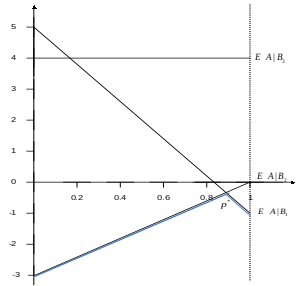
\includegraphics[width=60mm]{chapters/chapter5/figures/Picture1.png}
     \end{center}
     \caption{Representación función de pago}
\label{fig:func_pago}
\end{figure}
El valor óptimo de $p$ es aquel que maximiza los mínimos pagos esperados  por A. Vemos en el gráfico que este valor de $p$ se encuentra en el punto de corte entre las rectas  y  Resolviendo la ecuación: $-p+5(1-p)=-3(1-p)$ se obtiene que $p^*=\frac{8}{9}$.
\\
Si sustituimos en cualquiera de estas ecuaciones $p^*$, tendremos la cantidad que A espera ganar si juega con su estrategia óptima: $E(A^*|B_1)=E(A^*|B_2)=-\frac{3}{9}=v$. 
\\
\vspace{2mm}
La solución para este primer agente es $P^*=(\frac{8}{9},\frac{1}{9})$, siendo el valor del juego $-\frac{3}{9}$.
\\
\vspace{2mm}
Si nos fijamos en el gráfico podemos observar que $E(A^*|B_3)>v$ esto es, si A juega con su estrategia óptima, B no debe elegir la opción  ya que empeoraría su resultado esperado, mejorando la posición de $A$. Esto supone que la estrategia mixta de $B$ es: $Q=(q,1-q,0)$ con $q \in [0,1]$. 
\\
La función de pago esperado de este agente viene dada por:
\begin{center}
    $E(B|A_1)=-q$\\
    $E(B|A_2)=5q-3(1-q)$\\
\end{center}

Y su representación gráfica es (figura \ref{fig:func_pago2}):
\\
\begin{figure}[h]
     \begin{center}
         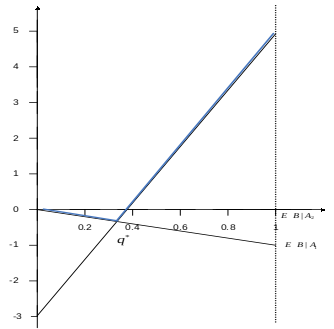
\includegraphics[width=60mm]{chapters/chapter5/figures/Picture2.png}
     \end{center}
     \caption{Representación función de pago esperado}
\label{fig:func_pago2}
\end{figure}
El valor óptimo de $q$ es aquel que minimice los máximos pagos esperados de $B$. Vemos en el gráfico que este valor de $q$ se encuentra en el punto de corte entre las dos rectas. Resolviendo la ecuación: $-q=5q-3(1-q)$ se obtiene que $q^*=\frac{1}{3}$.\\
\vspace{2mm}
Si sustituimos en cualquiera de las ecuaciones  tenemos la cantidad que B espera ganar si juega con su estrategia óptima: $E(B^*|A_1)=E(B^*|A_2)=-\frac{3}{9}=v$; cantidad que, evidentemente, coincide con la esperada por  A.
\\
\vspace{2mm}
La solución para el segundo agente es $Q^*=(\frac{1}{3},\frac{2}{3},0)$
\\
\vspace{2mm}
Antes de terminar el ejercicio, volvamos a la representación gráfica de la función de pago esperado por el agente A. En esta figura podemos observar que la recta que representa el pago esperado por A si B elige la alternativa $B_3$, esta, para cualquier valor de $p \in [0,1]$, por encima de la recta que representa dichos pagos esperados si B elige $B_2$.
\\
\begin{center}
    $E(A|B_3)>E(A|B_2) \: \forall p \in [0,1]$\\
\end{center}
Esto se debe a que la estrategia $B_3$ esta estrictamente dominada por $B_2$, ya que $r_{i2}<r_{i3} \: \forall i$,  dominación que no hemos comprobado y que simplifica el cálculo del resultado óptimo del juego, ya que reduce la dimensión de la matriz de pagos sin alterar la solución óptima. Podríamos haber resuelto un juego de dimensión (2x2) en vez de uno de dimensión (2x3).
\\
Interpretando la solución, diremos que los participantes juegan de forma óptima si, en el caso del agente $A$, utiliza, de cada nueve veces que juegue, ocho la primera estrategia y una la segunda; en el caso de $B$, si juega el 33.3\% de las ocasiones con la primera, el 66.6\% restante con la segunda y nunca con la tercera. Jugando así $B$ espera recibir de media de $A$ la cantidad de $\frac{3}{9}$.
\item En la matriz de pagos hay elementos negativos, por lo cual para construir el programa lineal que permita obtener la solución del juego, debemos sumar una constante, por ejemplo $k=3$ para garantizar que el valor del juego es positivo. No obstante, observe el lector que ya hemos resuelto el juego y sabemos que $v=-\frac{3}{9}$con lo cual bastaría sumar cualquier cantidad mayor que $\frac{3}{9}$ para cumplir este requisito.
La nueva matriz quedará:\\
\begin{center}
  $  \begin{pmatrix}
    2 & 3 & 6\\
    8 & 0 & 7
    \end{pmatrix}$\\
\end{center}
Siendo el valor del juego correspondiente a esta matriz $v'=v+3>0$
Si el agente $B$ elige sus estrategias según su estrategia mixta óptima $Q^*=(q_1,q_2,q_3)$  el pago que será espera realizar, con independencia de la estrategia por la que opte él, agente $A$, será como mucho el valor del juego, esto es:
\begin{center}
    $E(B|A_1)=2q_1+3q_2+6q_3\leq v'$\\
    $E(B|A_2)=8q_1+7q_3\leq v'$ \\
\end{center}
Si dividimos por $v'$ los dos miembros de estas desigualdades tendremos:
\\
\begin{center}
    $2\dfrac{q_1}{v'}+3\dfrac{q_2}{v'}+6\dfrac{q_3}{v'}\leq 1 $\\
    $8\dfrac{q_1}{v'}+7\dfrac{q_3}{v'}\leq 1$
\end{center}
Llamando $y_1=\frac{q1}{v'},y_2=\frac{q_2}{v'},y_3=\frac{q_3}{v'}$ y sustituyendo en las expresiones anteriores.
\begin{center}
    $2y_1+3y_2+6y_3\leq 1$\\
    $8y_1+7y_3\leq 1$\\
\end{center}

Siendo $y_j\geq 0$ para todo $j$, ya que $v>0$ y $q_j\geq 0$.
El valor del juego $v'$ podemos expresarlo en función de las nuevas variables $y_j$ ya que\\ 
\begin{center}
    $$\sum_{j=1}^{3} y_j = \frac{q_1}{v'}+\frac{q_2}{v'}+\frac{q_3}{v'}=\frac{1}{v'}(q_1+q_2+q_3)=\frac{1}{v'}$$\\
\end{center}
Como el objetivo del agente B es minimizar el valor del juego, lo conseguirá cuando $y_1+y_2+y_3$ alcance el máximo valor. De esta forma, el problema de decisión para el agente B se reduce a resolver el siguiente programa de optimización matemática:\\

\begin{center}
    Máx    $(y_1+y_2+y_3)$\\
    s.a $\quad 2y_1+3y_2+6y_3\leq 1$\\
    $8y_1+7y_3\leq 1$ \\
    $y_1\geq 0 \: y_2\geq 0 \: y_3\geq 0$\\
\end{center}


Recordando que al resolver obtenemos el valor $v'$, siendo el valor del juego mismo planteado originalmente $v=v-3$.
\end{enumerate}

